\PassOptionsToPackage{unicode=true}{hyperref} % options for packages loaded elsewhere
\PassOptionsToPackage{hyphens}{url}
%
\documentclass[]{article}
\usepackage{lmodern}
\usepackage{amssymb,amsmath}
\usepackage{ifxetex,ifluatex}
\usepackage{fixltx2e} % provides \textsubscript
\ifnum 0\ifxetex 1\fi\ifluatex 1\fi=0 % if pdftex
  \usepackage[T1]{fontenc}
  \usepackage[utf8]{inputenc}
  \usepackage{textcomp} % provides euro and other symbols
\else % if luatex or xelatex
  \usepackage{unicode-math}
  \defaultfontfeatures{Ligatures=TeX,Scale=MatchLowercase}
\fi
% use upquote if available, for straight quotes in verbatim environments
\IfFileExists{upquote.sty}{\usepackage{upquote}}{}
% use microtype if available
\IfFileExists{microtype.sty}{%
\usepackage[]{microtype}
\UseMicrotypeSet[protrusion]{basicmath} % disable protrusion for tt fonts
}{}
\IfFileExists{parskip.sty}{%
\usepackage{parskip}
}{% else
\setlength{\parindent}{0pt}
\setlength{\parskip}{6pt plus 2pt minus 1pt}
}
\usepackage{hyperref}
\hypersetup{
            pdftitle={IDDAP Visuals and Stats},
            pdfauthor={Elnaz Ghajar-Rahimi (eg8cm)},
            pdfborder={0 0 0},
            breaklinks=true}
\urlstyle{same}  % don't use monospace font for urls
\usepackage[margin=1in]{geometry}
\usepackage{color}
\usepackage{fancyvrb}
\newcommand{\VerbBar}{|}
\newcommand{\VERB}{\Verb[commandchars=\\\{\}]}
\DefineVerbatimEnvironment{Highlighting}{Verbatim}{commandchars=\\\{\}}
% Add ',fontsize=\small' for more characters per line
\usepackage{framed}
\definecolor{shadecolor}{RGB}{248,248,248}
\newenvironment{Shaded}{\begin{snugshade}}{\end{snugshade}}
\newcommand{\AlertTok}[1]{\textcolor[rgb]{0.94,0.16,0.16}{#1}}
\newcommand{\AnnotationTok}[1]{\textcolor[rgb]{0.56,0.35,0.01}{\textbf{\textit{#1}}}}
\newcommand{\AttributeTok}[1]{\textcolor[rgb]{0.77,0.63,0.00}{#1}}
\newcommand{\BaseNTok}[1]{\textcolor[rgb]{0.00,0.00,0.81}{#1}}
\newcommand{\BuiltInTok}[1]{#1}
\newcommand{\CharTok}[1]{\textcolor[rgb]{0.31,0.60,0.02}{#1}}
\newcommand{\CommentTok}[1]{\textcolor[rgb]{0.56,0.35,0.01}{\textit{#1}}}
\newcommand{\CommentVarTok}[1]{\textcolor[rgb]{0.56,0.35,0.01}{\textbf{\textit{#1}}}}
\newcommand{\ConstantTok}[1]{\textcolor[rgb]{0.00,0.00,0.00}{#1}}
\newcommand{\ControlFlowTok}[1]{\textcolor[rgb]{0.13,0.29,0.53}{\textbf{#1}}}
\newcommand{\DataTypeTok}[1]{\textcolor[rgb]{0.13,0.29,0.53}{#1}}
\newcommand{\DecValTok}[1]{\textcolor[rgb]{0.00,0.00,0.81}{#1}}
\newcommand{\DocumentationTok}[1]{\textcolor[rgb]{0.56,0.35,0.01}{\textbf{\textit{#1}}}}
\newcommand{\ErrorTok}[1]{\textcolor[rgb]{0.64,0.00,0.00}{\textbf{#1}}}
\newcommand{\ExtensionTok}[1]{#1}
\newcommand{\FloatTok}[1]{\textcolor[rgb]{0.00,0.00,0.81}{#1}}
\newcommand{\FunctionTok}[1]{\textcolor[rgb]{0.00,0.00,0.00}{#1}}
\newcommand{\ImportTok}[1]{#1}
\newcommand{\InformationTok}[1]{\textcolor[rgb]{0.56,0.35,0.01}{\textbf{\textit{#1}}}}
\newcommand{\KeywordTok}[1]{\textcolor[rgb]{0.13,0.29,0.53}{\textbf{#1}}}
\newcommand{\NormalTok}[1]{#1}
\newcommand{\OperatorTok}[1]{\textcolor[rgb]{0.81,0.36,0.00}{\textbf{#1}}}
\newcommand{\OtherTok}[1]{\textcolor[rgb]{0.56,0.35,0.01}{#1}}
\newcommand{\PreprocessorTok}[1]{\textcolor[rgb]{0.56,0.35,0.01}{\textit{#1}}}
\newcommand{\RegionMarkerTok}[1]{#1}
\newcommand{\SpecialCharTok}[1]{\textcolor[rgb]{0.00,0.00,0.00}{#1}}
\newcommand{\SpecialStringTok}[1]{\textcolor[rgb]{0.31,0.60,0.02}{#1}}
\newcommand{\StringTok}[1]{\textcolor[rgb]{0.31,0.60,0.02}{#1}}
\newcommand{\VariableTok}[1]{\textcolor[rgb]{0.00,0.00,0.00}{#1}}
\newcommand{\VerbatimStringTok}[1]{\textcolor[rgb]{0.31,0.60,0.02}{#1}}
\newcommand{\WarningTok}[1]{\textcolor[rgb]{0.56,0.35,0.01}{\textbf{\textit{#1}}}}
\usepackage{graphicx,grffile}
\makeatletter
\def\maxwidth{\ifdim\Gin@nat@width>\linewidth\linewidth\else\Gin@nat@width\fi}
\def\maxheight{\ifdim\Gin@nat@height>\textheight\textheight\else\Gin@nat@height\fi}
\makeatother
% Scale images if necessary, so that they will not overflow the page
% margins by default, and it is still possible to overwrite the defaults
% using explicit options in \includegraphics[width, height, ...]{}
\setkeys{Gin}{width=\maxwidth,height=\maxheight,keepaspectratio}
\setlength{\emergencystretch}{3em}  % prevent overfull lines
\providecommand{\tightlist}{%
  \setlength{\itemsep}{0pt}\setlength{\parskip}{0pt}}
\setcounter{secnumdepth}{0}
% Redefines (sub)paragraphs to behave more like sections
\ifx\paragraph\undefined\else
\let\oldparagraph\paragraph
\renewcommand{\paragraph}[1]{\oldparagraph{#1}\mbox{}}
\fi
\ifx\subparagraph\undefined\else
\let\oldsubparagraph\subparagraph
\renewcommand{\subparagraph}[1]{\oldsubparagraph{#1}\mbox{}}
\fi

% set default figure placement to htbp
\makeatletter
\def\fps@figure{htbp}
\makeatother


\title{IDDAP Visuals and Stats}
\author{Elnaz Ghajar-Rahimi (eg8cm)}
\date{3/23/2020}

\begin{document}
\maketitle

Loading libraries + mock sheet (pf for short)

\begin{Shaded}
\begin{Highlighting}[]
\KeywordTok{library}\NormalTok{(dplyr)}
\end{Highlighting}
\end{Shaded}

\begin{verbatim}
## 
## Attaching package: 'dplyr'
\end{verbatim}

\begin{verbatim}
## The following objects are masked from 'package:stats':
## 
##     filter, lag
\end{verbatim}

\begin{verbatim}
## The following objects are masked from 'package:base':
## 
##     intersect, setdiff, setequal, union
\end{verbatim}

\begin{Shaded}
\begin{Highlighting}[]
\KeywordTok{library}\NormalTok{(ggplot2)}
\KeywordTok{library}\NormalTok{(tidyr)}
\KeywordTok{library}\NormalTok{(RColorBrewer)}

\NormalTok{pf=}\KeywordTok{read.csv}\NormalTok{(}\StringTok{"/Users/jessmahoney/Desktop/capstoneR/IDDAP2020/mdata.csv"}\NormalTok{,}\DataTypeTok{stringsAsFactors=}\OtherTok{FALSE}\NormalTok{)}
\end{Highlighting}
\end{Shaded}

Data visualizations

Antibiotic counts

\begin{Shaded}
\begin{Highlighting}[]
\CommentTok{#Bar Graph}
\KeywordTok{ggplot}\NormalTok{(pf,}\KeywordTok{aes}\NormalTok{(}\DataTypeTok{x=}\NormalTok{Antibiotic))}\OperatorTok{+}\KeywordTok{geom_bar}\NormalTok{(}\DataTypeTok{fill=}\KeywordTok{brewer.pal}\NormalTok{(}\DecValTok{7}\NormalTok{,}\StringTok{"Set1"}\NormalTok{))}\OperatorTok{+}\KeywordTok{ylab}\NormalTok{(}\StringTok{"Numer of Patients Taking Antibiotic"}\NormalTok{)}
\end{Highlighting}
\end{Shaded}

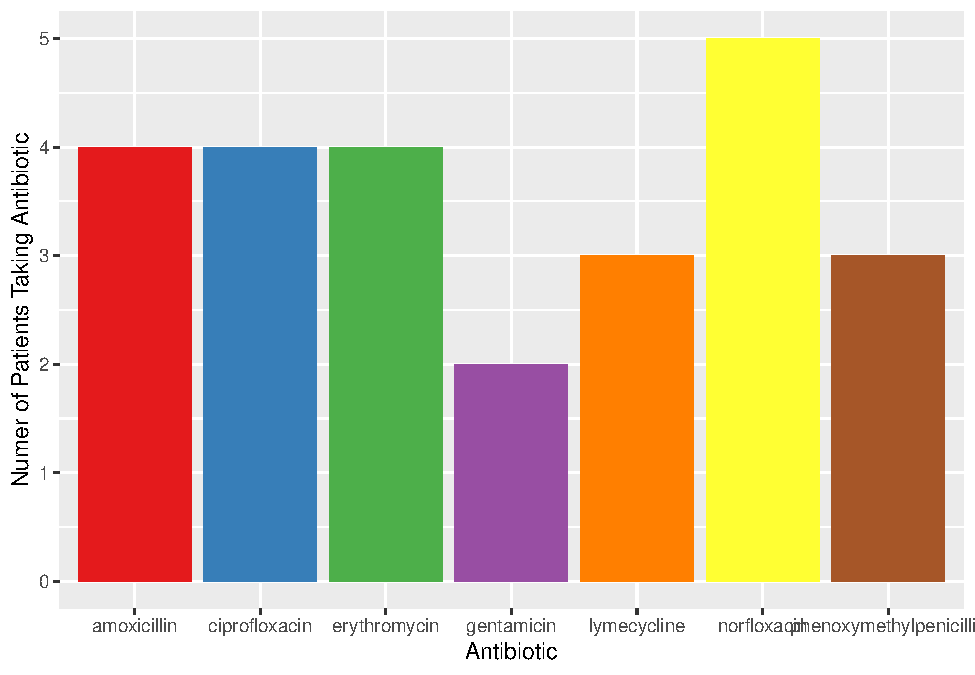
\includegraphics{IDDAP_Visuals_Stat_files/figure-latex/unnamed-chunk-2-1.pdf}

\begin{Shaded}
\begin{Highlighting}[]
\CommentTok{#NOTE: the first argument in brewer.pal is the number of categories (ex the numer of antibiotic types)}

\CommentTok{#Tabulate}
\KeywordTok{table}\NormalTok{(pf}\OperatorTok{$}\NormalTok{Antibiotic)}
\end{Highlighting}
\end{Shaded}

\begin{verbatim}
## 
##             amoxicillin           ciprofloxacin            erythromycin 
##                       4                       4                       4 
##              gentamicin             lymecycline             norfloxacin 
##                       2                       3                       5 
## phenoxymethylpenicillin 
##                       3
\end{verbatim}

Age, weight, and risk of readmission

Percent bar graph: antibiotic and resistant organism

\begin{Shaded}
\begin{Highlighting}[]
\KeywordTok{ggplot}\NormalTok{(pf,}\KeywordTok{aes}\NormalTok{(}\DataTypeTok{x=}\NormalTok{Antibiotic,}\DataTypeTok{fill=}\NormalTok{Resistant.Organism..Y.N.))}\OperatorTok{+}\KeywordTok{geom_bar}\NormalTok{(}\DataTypeTok{position=}\StringTok{"fill"}\NormalTok{)}\OperatorTok{+}\KeywordTok{labs}\NormalTok{(}\DataTypeTok{x=}\StringTok{"Antibiotic"}\NormalTok{,}\DataTypeTok{y=}\StringTok{"Number of Patients"}\NormalTok{)}\OperatorTok{+}\KeywordTok{theme}\NormalTok{(}\DataTypeTok{axis.text.x=}\KeywordTok{element_text}\NormalTok{(}\DataTypeTok{angle=}\DecValTok{30}\NormalTok{),}\DataTypeTok{plot.title=}\KeywordTok{element_text}\NormalTok{(}\DataTypeTok{hjust=}\FloatTok{0.5}\NormalTok{))}
\end{Highlighting}
\end{Shaded}

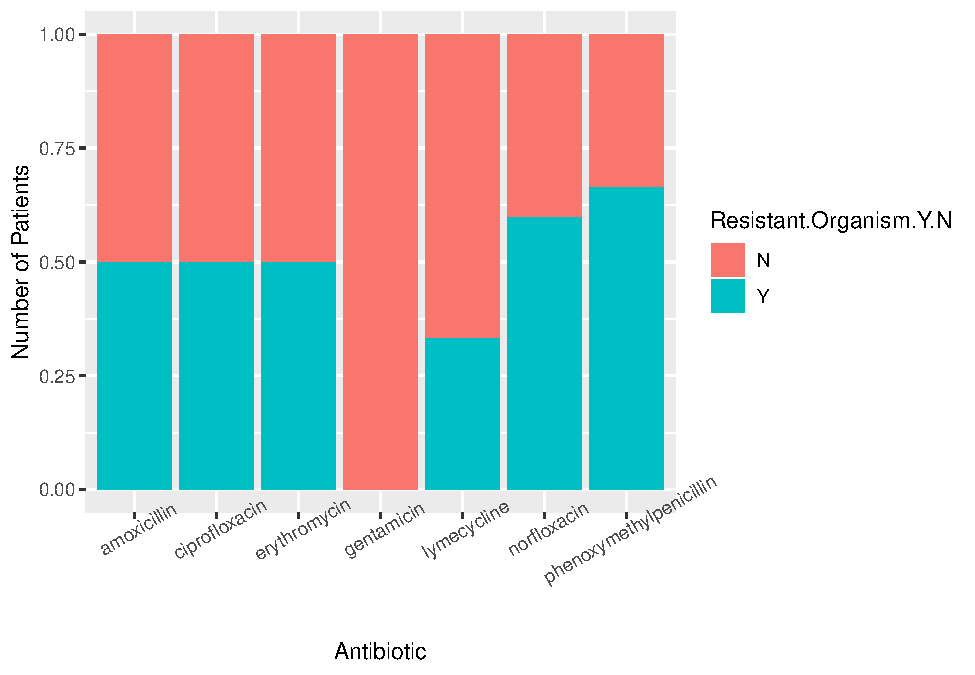
\includegraphics{IDDAP_Visuals_Stat_files/figure-latex/unnamed-chunk-3-1.pdf}

\hypertarget{statistics}{%
\subsubsection{Statistics}\label{statistics}}

Average height and age of patient taking each antibiotic

\begin{Shaded}
\begin{Highlighting}[]
\KeywordTok{aggregate}\NormalTok{(pf[,}\KeywordTok{c}\NormalTok{(}\DecValTok{3}\NormalTok{,}\DecValTok{4}\NormalTok{)], }\KeywordTok{list}\NormalTok{(pf}\OperatorTok{$}\NormalTok{Antibiotic),mean,}\DataTypeTok{na.rm=}\NormalTok{T)}
\end{Highlighting}
\end{Shaded}

\begin{verbatim}
##                   Group.1      Age Height..m.
## 1             amoxicillin 48.25000   1.750000
## 2           ciprofloxacin 59.50000   1.692500
## 3            erythromycin 69.25000   1.600000
## 4              gentamicin 69.00000   1.810000
## 5             lymecycline 54.33333   1.693333
## 6             norfloxacin 48.40000   1.700000
## 7 phenoxymethylpenicillin 73.33333   1.663333
\end{verbatim}

\hypertarget{extra-stuff}{%
\subsubsection{Extra Stuff}\label{extra-stuff}}

Making Risk of readmisison binary (Y=1, N=0)

\begin{Shaded}
\begin{Highlighting}[]
\NormalTok{risk=}\OtherTok{NULL}

\ControlFlowTok{for}\NormalTok{ (i }\ControlFlowTok{in} \DecValTok{1}\OperatorTok{:}\KeywordTok{nrow}\NormalTok{(pf))}
\NormalTok{\{}
  \ControlFlowTok{if}\NormalTok{ (pf[i,}\DecValTok{9}\NormalTok{]}\OperatorTok{==}\StringTok{"N"}\NormalTok{) \{risk[i]=}\DecValTok{0}\NormalTok{\}}
  \ControlFlowTok{else}\NormalTok{ \{risk[i]=}\DecValTok{1}\NormalTok{\}}
\NormalTok{\}}


\CommentTok{#This just adds it to a new column so that I could check if the counts were correct}
\NormalTok{revised_pf=}\KeywordTok{data.frame}\NormalTok{(pf,risk)}
\CommentTok{#View(revised_pf)}

\CommentTok{#if ("High.Risk.of.Readmission"=="Y") \{\}}
\KeywordTok{ggplot}\NormalTok{(pf,}\KeywordTok{aes}\NormalTok{(}\DataTypeTok{x=}\NormalTok{Age,}\DataTypeTok{y=}\NormalTok{risk))}\OperatorTok{+}\KeywordTok{geom_point}\NormalTok{()}
\end{Highlighting}
\end{Shaded}

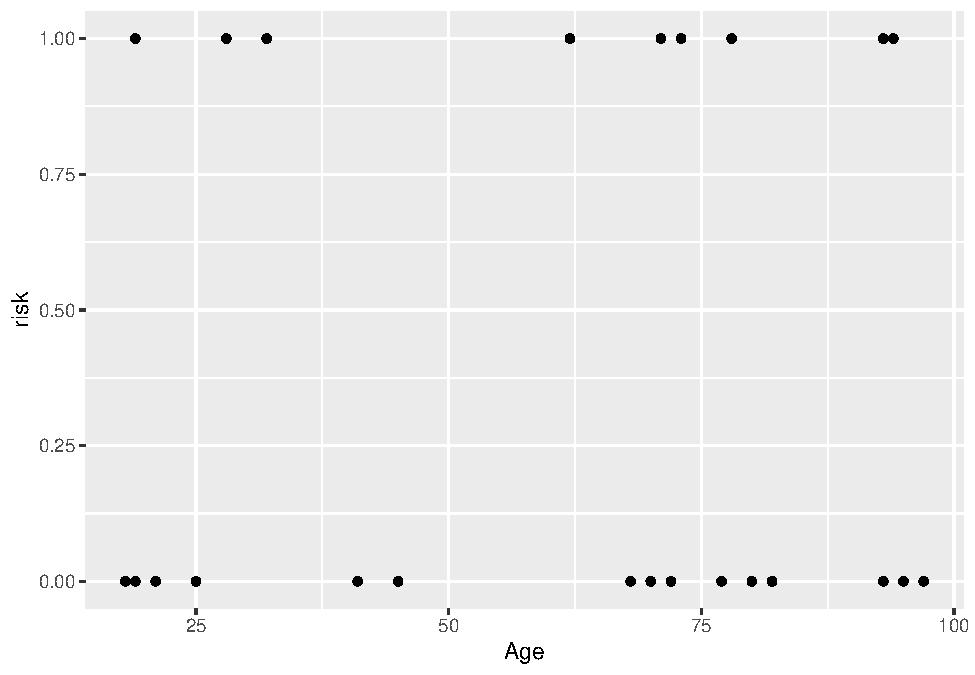
\includegraphics{IDDAP_Visuals_Stat_files/figure-latex/unnamed-chunk-5-1.pdf}

\textbf{Accounting for all spellings of Yes/No }

\begin{itemize}
\tightlist
\item
  pf\_new was created to prevent overriding of original file
\item
  Risk is the corrected version of ``High Risk of Readmission''
\item
  Resistance is the corrected version of Resistant Organism
\end{itemize}

\begin{Shaded}
\begin{Highlighting}[]
\CommentTok{#Correct resistance}
\NormalTok{pf_new=pf}
\NormalTok{pf_new=pf_new}\OperatorTok
\KeywordTok{mutate}\NormalTok{(}\DataTypeTok{Resistance=}\KeywordTok{ifelse}\NormalTok{(}\KeywordTok{grepl}\NormalTok{(}\KeywordTok{paste}\NormalTok{(}\KeywordTok{c}\NormalTok{(}\StringTok{"Y"}\NormalTok{,}\StringTok{"YES"}\NormalTok{,}\StringTok{"YEs"}\NormalTok{,}\StringTok{"Yes"}\NormalTok{,}\StringTok{"y"}\NormalTok{,}\StringTok{"yE"}\NormalTok{,}\StringTok{"yES"}\NormalTok{,}\StringTok{"yes"}\NormalTok{),}\DataTypeTok{collapse=}\StringTok{"|"}\NormalTok{),Resistant.Organism..Y.N.),}\StringTok{"Y"}\NormalTok{,}
\KeywordTok{ifelse}\NormalTok{(}\KeywordTok{grepl}\NormalTok{(}\KeywordTok{paste}\NormalTok{(}\KeywordTok{c}\NormalTok{(}\StringTok{"N"}\NormalTok{,}\StringTok{"NO"}\NormalTok{,}\StringTok{"No"}\NormalTok{,}\StringTok{"nO"}\NormalTok{,}\StringTok{"no"}\NormalTok{),}\DataTypeTok{collapse=}\StringTok{"|"}\NormalTok{),Resistant.Organism..Y.N.),}\StringTok{"N"}\NormalTok{,}\StringTok{"Unrecognized Input"}
\NormalTok{)))}

\CommentTok{#Correct risk of readmission}
\NormalTok{pf_new=pf_new}\OperatorTok
\KeywordTok{mutate}\NormalTok{(}\DataTypeTok{Risk=}\KeywordTok{ifelse}\NormalTok{(}\KeywordTok{grepl}\NormalTok{(}\KeywordTok{paste}\NormalTok{(}\KeywordTok{c}\NormalTok{(}\StringTok{"Y"}\NormalTok{,}\StringTok{"YES"}\NormalTok{,}\StringTok{"YEs"}\NormalTok{,}\StringTok{"Yes"}\NormalTok{,}\StringTok{"y"}\NormalTok{,}\StringTok{"yE"}\NormalTok{,}\StringTok{"yES"}\NormalTok{,}\StringTok{"yes"}\NormalTok{),}\DataTypeTok{collapse=}\StringTok{"|"}\NormalTok{),High.Risk.of.Readmission),}\StringTok{"Y"}\NormalTok{,}
\KeywordTok{ifelse}\NormalTok{(}\KeywordTok{grepl}\NormalTok{(}\KeywordTok{paste}\NormalTok{(}\KeywordTok{c}\NormalTok{(}\StringTok{"N"}\NormalTok{,}\StringTok{"NO"}\NormalTok{,}\StringTok{"No"}\NormalTok{,}\StringTok{"nO"}\NormalTok{,}\StringTok{"no"}\NormalTok{),}\DataTypeTok{collapse=}\StringTok{"|"}\NormalTok{),High.Risk.of.Readmission),}\StringTok{"N"}\NormalTok{,}\StringTok{"Unrecognized Input"}
\NormalTok{)))}
\end{Highlighting}
\end{Shaded}

\begin{Shaded}
\begin{Highlighting}[]
\CommentTok{#Correct gender spellings}
\NormalTok{pf_new=pf_new}\OperatorTok
\KeywordTok{mutate}\NormalTok{(}\DataTypeTok{Sex=}\KeywordTok{ifelse}\NormalTok{(}\KeywordTok{grepl}\NormalTok{(}\KeywordTok{paste}\NormalTok{(}\KeywordTok{c}\NormalTok{(}\StringTok{"F"}\NormalTok{,}\StringTok{"f"}\NormalTok{),}\DataTypeTok{collapse=}\StringTok{"|"}\NormalTok{),Gender..M.F.),}\StringTok{"F"}\NormalTok{,}
\KeywordTok{ifelse}\NormalTok{(}\KeywordTok{grepl}\NormalTok{(}\KeywordTok{paste}\NormalTok{(}\KeywordTok{c}\NormalTok{(}\StringTok{"M"}\NormalTok{,}\StringTok{"m"}\NormalTok{),}\DataTypeTok{collapse=}\StringTok{"|"}\NormalTok{),Gender..M.F.),}\StringTok{"M"}\NormalTok{,}\StringTok{"Unrecognized Input"}
\NormalTok{)))}

\CommentTok{#View to check. It works!}
\KeywordTok{View}\NormalTok{(pf_new)}
\end{Highlighting}
\end{Shaded}

\end{document}
